\chapter{Results}
\label{s:results}

\section{Euler}
One of the first tests for an ODE solver is whether it handles harmonic oscillations properly. The simple oscillations (shown in \ref{eq:osceq} with their analytical solutions) can be implemented as a matrix vector equation (\ref{eq:oscmatrix}), which represents two uncoupled oscillations of different frequencies. Besides the matrix of constants, the solver also requires initial values. For the first oscillation the initial position is non-zero, for the second oscillation the initial velocity is non-zero. 

\begin{align}
\label{eq:osceq} \nonumber
x_{0} '' &= - x_{0} \\
x_{2} '' &= -4 x_{2} \\ \nonumber
\\ \nonumber
\label{eq:osceqsol} \nonumber
x_{0}(t)  &= 50 \cos{(t)} \\ \nonumber
x_{2}(t)  &= 25 \sin{(2t)} \\ \nonumber
\end{align}


\begin{equation}
\label{eq:oscmatrix}
\vecb{x}' = \begin{bmatrix} 
0 & 1 & 0 & 0 \\
-1 & 0 & 0 & 0 \\
0 & 0 & 0 & 1 \\
0 & 0 & -4 & 0 \\
\end{bmatrix} \vecb{x} 
\hspace{20pt} \text{with} \hspace{20pt} 
\vecb{x}(t = 0) =\begin{bmatrix} 50 \\ 0 \\ 0 \\ 50 \end{bmatrix} 
\end{equation}


\begin{figure}[h]
	\centering
	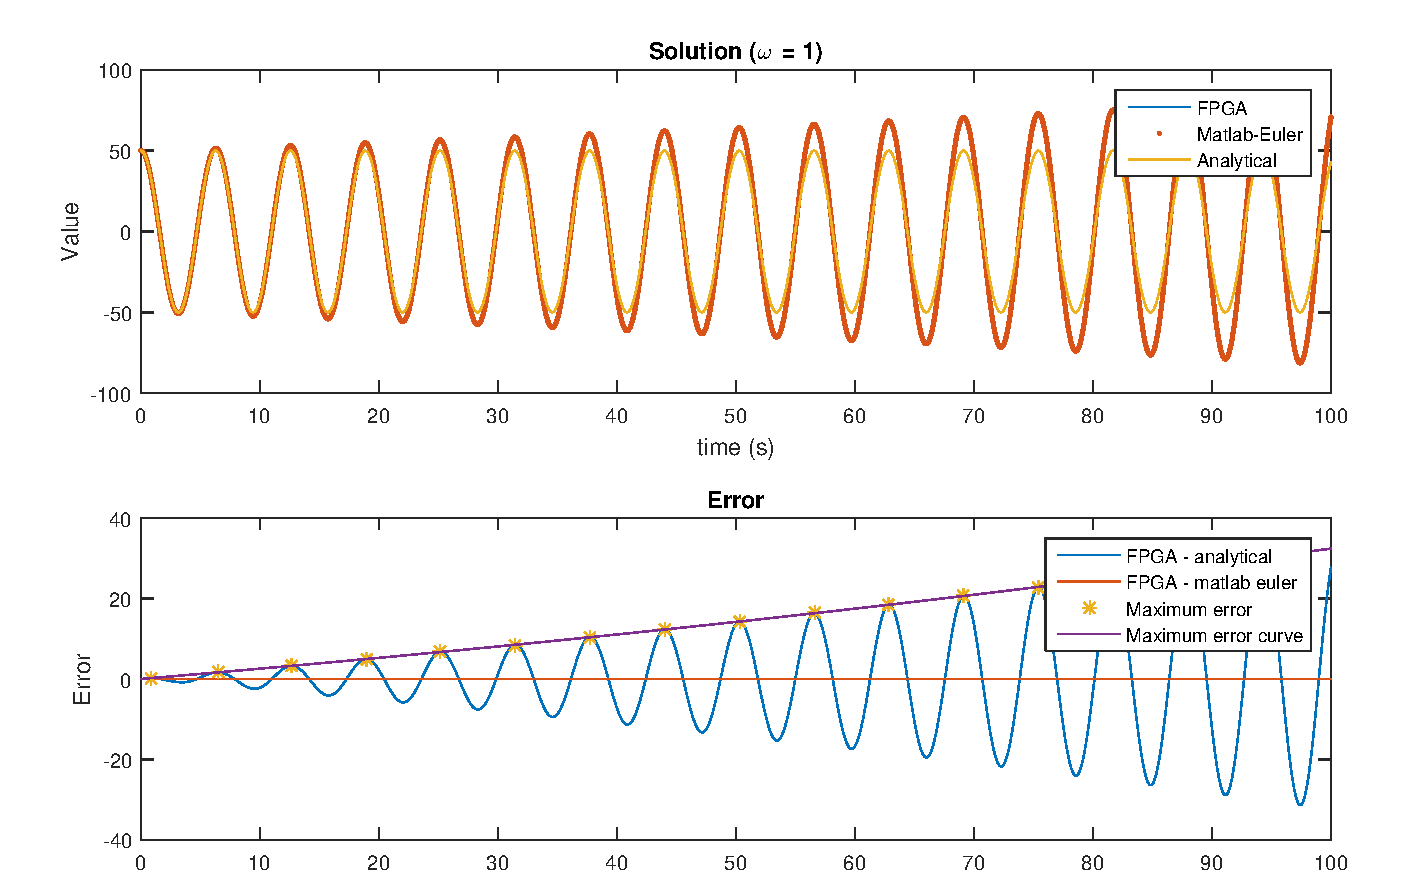
\includegraphics[width=\textwidth]{euler_o1_ts=0,01_os=1}
	\caption{Simple oscillation using Euler's method (h = 0.01)}
	\label{f:euler_o1_ts=0,01_os=1}
\end{figure}

\subsection{First oscillation}
The plots belonging to the first oscillation (\ref{f:euler_o1_ts=0,01_os=1}) depict three variations on solving the system. Firstly, it contains the solution generated by the FPGA. Secondly, it contains the result of the exact same combination of equation and solver, but implemented in \matlab{}. The only difference between the FPGA and \matlab{} implementation is the number representation. Therefore, if the FPGA solution starts to diverge from the \matlab{} solution the reason has to be the reduced accuracy of the 32-bit fixed point representation used in the FPGA. Internally, \matlab{} uses a (64-bit) double precision floating format \cite{MatlabFloat}, which is guaranteeing a precision of ~15 significant figures for almost all magnitudes supported by the IEEE 754 double precision floating point standard. Lastly, the plot contains the analytical solution of the problem.

The plot shows that the FPGA exhibits the expected behaviour of solving a simple oscillation with Euler's method. Due to the relatively large step size (h = 0.01) the approximation quickly diverges from the analytical solution. The curvature of the solution is always opposite in sign to the solution itself ($x'' = -x$), which results in a self-amplifying effect in the magnitude of the error: an exponential error growth. This was expected, as the exponential dependency was already derived by \cite{DE} in equation \ref{eq:euler_error}. However, this does show that Euler's method is a particularly bad integration scheme for a simple oscillation. It is possible to use \matlab{}s Curve Fitting Tool to fit the equation of the theoretical maximum error of Euler's method to the points of maximum error. After combining some constants, \ref{eq:euler_error} becomes equal to \ref{eq:euler_error_combined}. For $a = 49.75$ and $b = 0.00502$ this equation achieves a fit of $R^{2} = 1$, which is a perfect fit. The error plot and the curve fit of the maximum errors are shown in \ref{f:euler_o1_ts=0,01_os=1}.

\begin{equation}
\label{eq:euler_error_combined}
\text{error}_{\text{euler}}(t) = a (e^{b t} - 1)
\end{equation}

Lastly, the FPGA solution the solution of Euler's method implemented in \matlab{} shows that the error due to the fixed point number representation is clearly insignificant when compared to the intrinsic error in Euler's method: the maximum absolute difference between the two solutions is less than 6\e{-5}.

\subsubsection{Decreasing the time step - improving accuracy?}
The expectation based on \cite{DE} and equation \ref{eq:euler_error} is that the maximum error is indeed proportional to the time step, meaning that a hundred fold decrease of the time step also decreases the error by a factor 100. The maximum error at $t \approx 100$ for $h = 0.01$ was $\approx 30$, whereas the maximum error for $h = 0.0001$ is $\approx 0.2$, which is an improvement of $150 \times$, 50\% more than expected. However, even though the error relative to the analytical solution has decreased, the divergence from the \matlab{} implementation of Euler's algorithm has increased to 8\e{-4}, a factor of 13.
\begin{figure}[h]
	\centering
	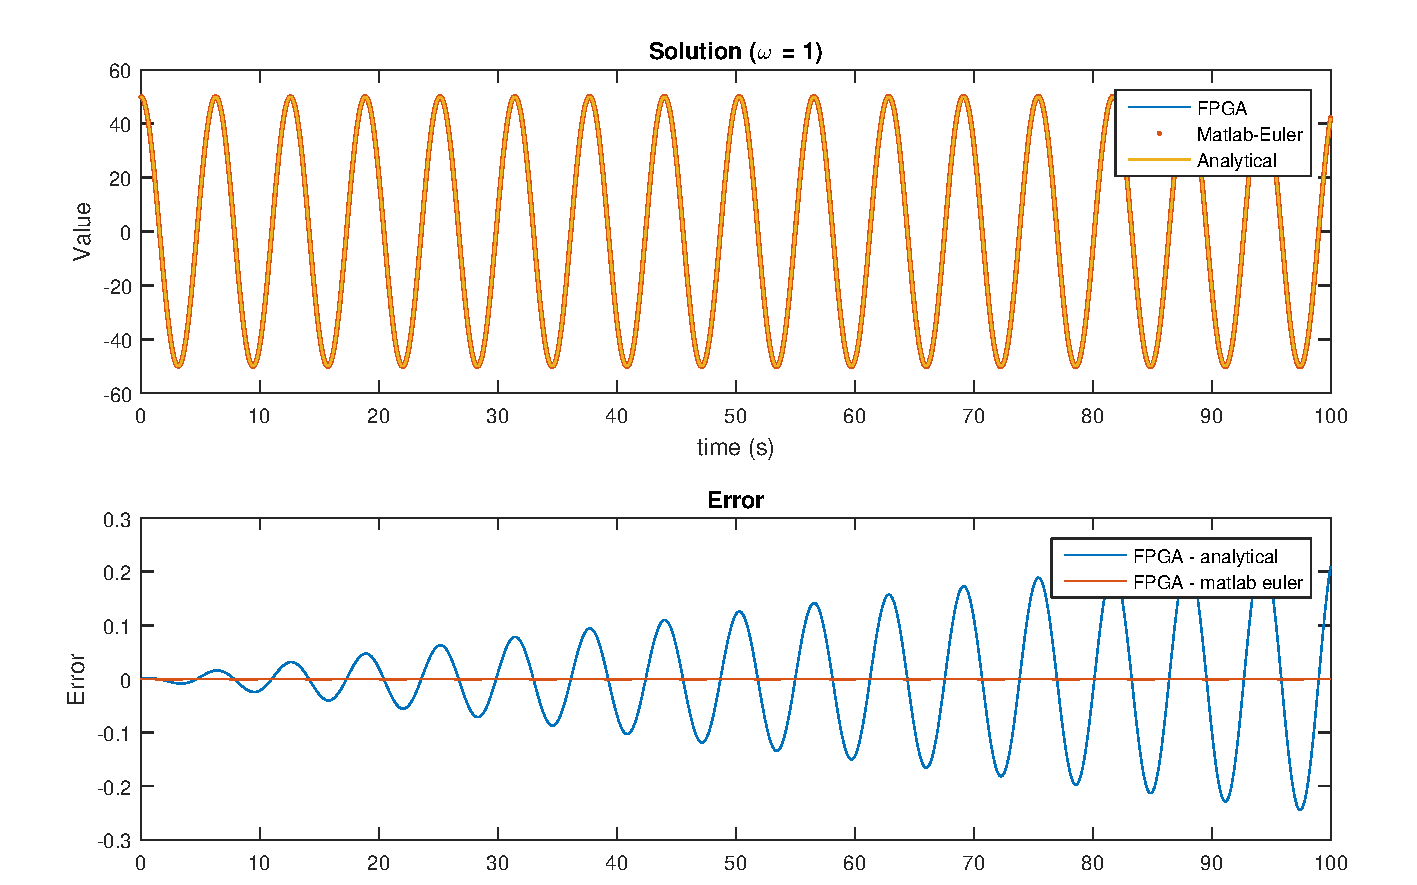
\includegraphics[width=\textwidth]{euler_o1_ts=0,0001_os=100}
	\caption{Simple oscillation using Euler's method with a lower time step (h = 0.0001)}
	\label{f:euler_o1_ts=0,0001_os=100}
\end{figure}


\subsection{First oscillation}



\subsection{Accuracy}
\subsection{Performance}

\section{Runge-Kutta (second order)}
\subsection{Accuracy}
\subsection{Performance}

\section{Runge-Kutta (fourth order)}

\section{Comparison with CPU implementations}
\section{Comparison with GPU implementations}





